%
% $RCSfile: hierarchical_model_view_controller.tex,v $
%
% Copyright (C) 2002-2008. Christian Heller.
%
% Permission is granted to copy, distribute and/or modify this document
% under the terms of the GNU Free Documentation License, Version 1.1 or
% any later version published by the Free Software Foundation; with no
% Invariant Sections, with no Front-Cover Texts and with no Back-Cover
% Texts. A copy of the license is included in the section entitled
% "GNU Free Documentation License".
%
% http://www.cybop.net
% - Cybernetics Oriented Programming -
%
% http://www.resmedicinae.org
% - Information in Medicine -
%
% Version: $Revision: 1.1 $ $Date: 2008-08-19 20:41:07 $ $Author: christian $
% Authors: Christian Heller <christian.heller@tuxtax.de>
%

\subsubsection{Hierarchical Model View Controller}
\label{hierarchical_model_view_controller_heading}
\index{Hierarchical Model View Controller Pattern}
\index{HMVC}
\index{Model View Controller Pattern}
\index{MVC}
\index{Composite Pattern}
\index{Layers Pattern}
\index{Chain of Responsibility Pattern}
\index{Presentation Layer}
\index{MVC Triad}
\index{Presentation Abstraction Control}
\index{PAC}
\index{PAC Agent}

There exist several extensions of the MVC pattern, one of them being the
\emph{Hierarchical Model View Controller} (HMVC) \cite{cai}. It combines the
patterns \emph{Composite} (section \ref{composite_heading}), \emph{Layers}
(section \ref{layers_heading}) and \emph{Chain of Responsibility} (section
\ref{chain_of_responsibility_heading}) into one conceptual architecture (figure
\ref{hmvc_figure}). This architecture divides the presentation layer into
hierarchical sections containing so-called \emph{MVC Triads}. The triads
conventionally consist of \emph{Model}, \emph{View} and \emph{Controller},
each. They communicate with each other by relating over their controller
object. Following the \emph{Layers} pattern, only neighbouring layers know from
each other.

\begin{figure}[ht]
    \begin{center}
        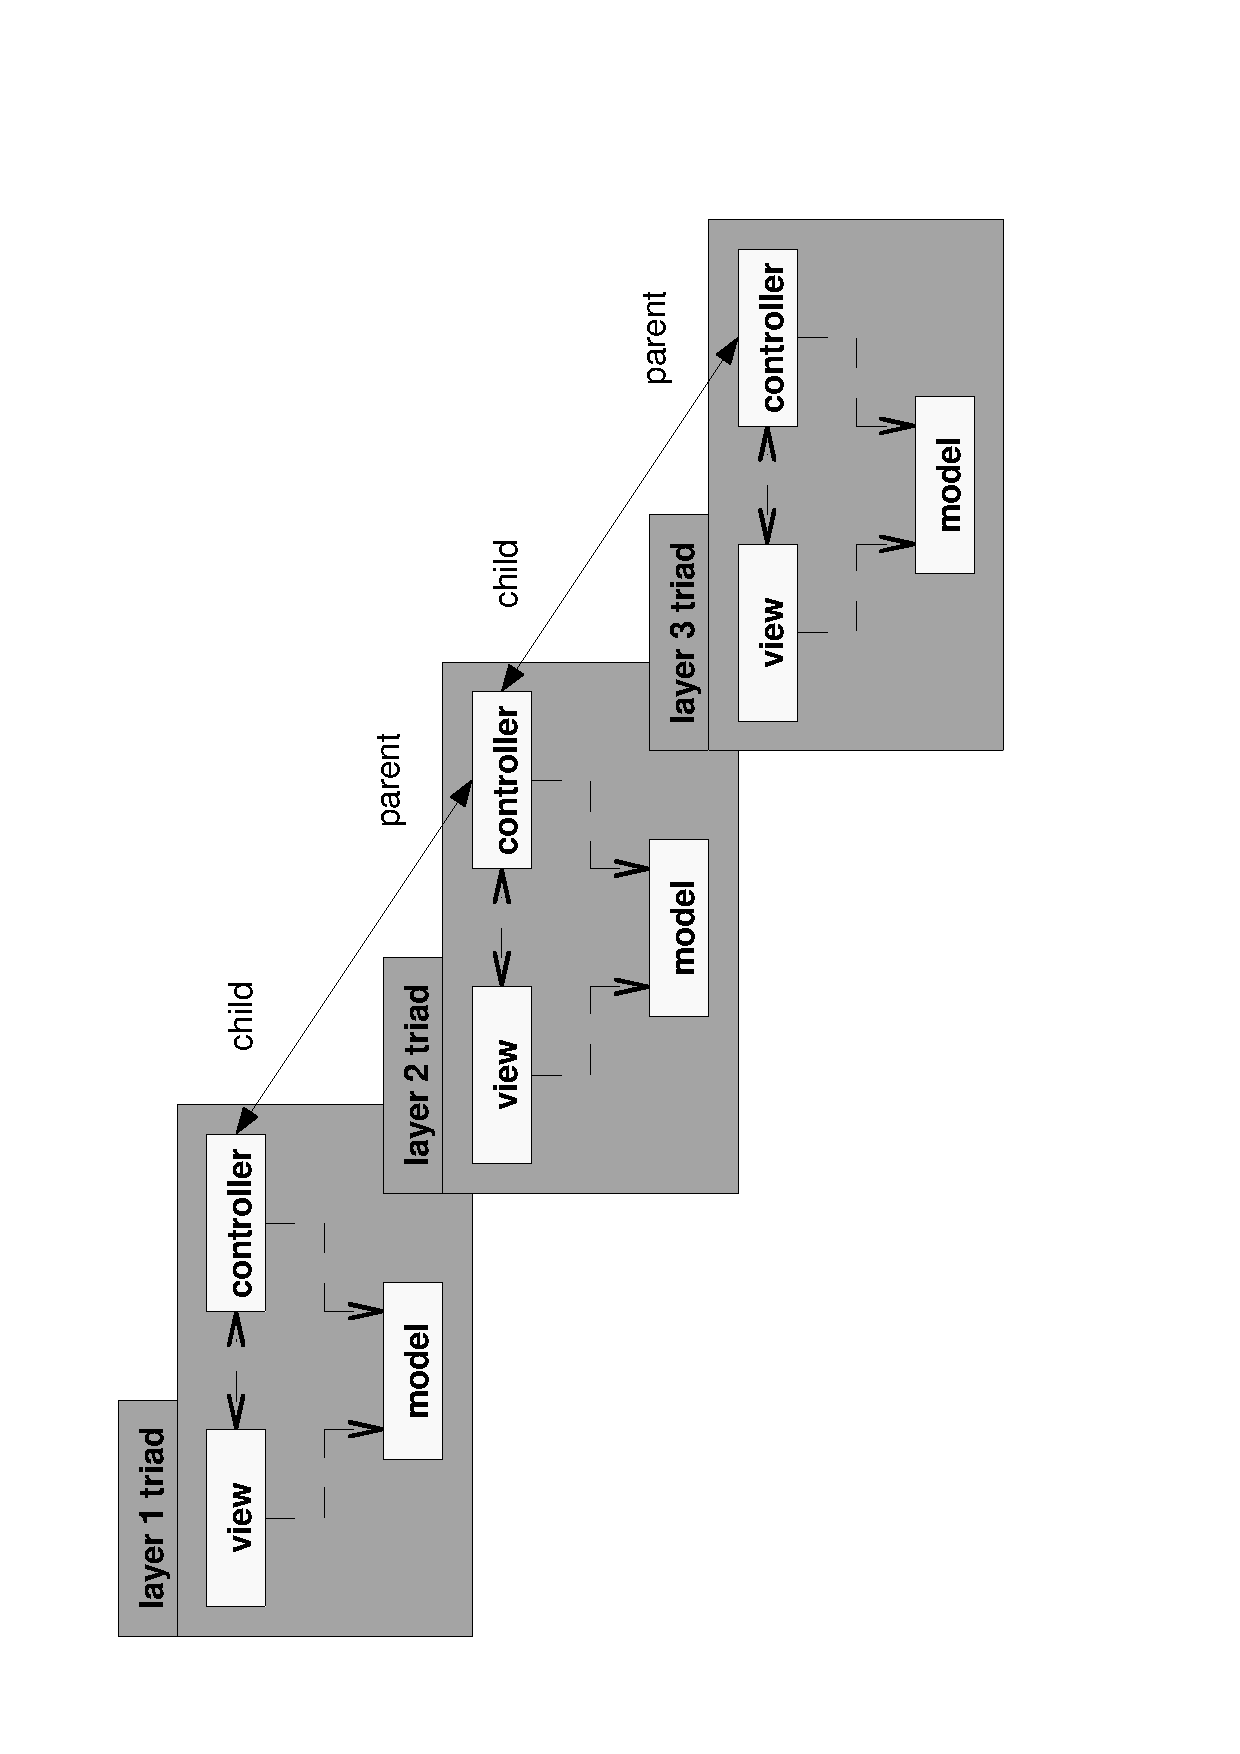
\includegraphics[scale=0.3,angle=-90]{graphic/hmvc.pdf}
        \caption{Hierarchical Model View Controller Pattern}
        \label{hmvc_figure}
    \end{center}
\end{figure}

As a practical example, the upper-most triad could represent a graphical
\emph{Dialogue} and the next lower one a \emph{Panel}. Being a container, too,
the panel could hold a third triad like for example a \emph{Button}. Events
occuring at the button are then normally processed by the corresponding
controller belonging to the button's triad. If, however, the button controller
cannot handle the event, that is forwarded along the chain of responsibility to
the controller of the higher-next layer. If also the panel controller does not
know how to handle the event, the final responsibility falls to the controller
of the dialogue's triad.

The HMVC is similar to the \emph{Presentation Abstraction Control} (PAC) pattern
\cite{buschmann}. A \emph{PAC Agent} is comparable to an \emph{HMVC Triad}.

Chapter \ref{knowledge_schema_heading} will apply the principle of
\emph{Hierarchy} not only to logic- (controller), but also to user interface-
(view), domain- and further models.
